\documentclass[crop,tikz,border=10px,convert=pdf2svg,multi=false]{standalone}
\usepackage[defaultsans]{opensans}
\usetikzlibrary{shapes,arrows,positioning}
\begin{document}
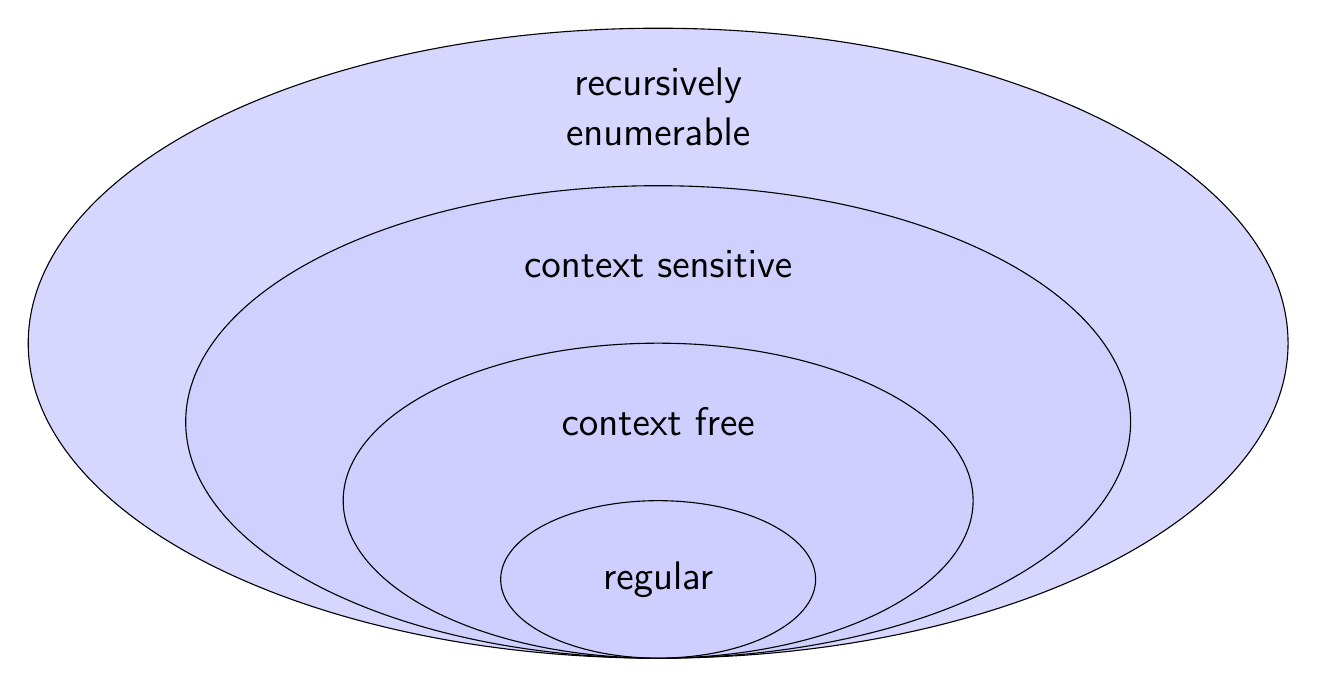
\begin{tikzpicture}[font=\Large\sffamily,
  block/.style = {fill=blue!20, minimum height=4em},
  mytext/.style = {draw=none, text centered, text width=12em, minimum height=4}]

  \begin{scope}
    \foreach \i/\n in {4/recursively enumerable,3/context sensitive,2/context free,1/regular}
    {
      \draw[block,fill opacity={\i * 0.2}] (0, {1 * \i}) ellipse ({2 * \i} and {1 * \i});
      \node[mytext] () at (0, {2 * \i - 1}) {\n};
    }
  \end{scope}


\end{tikzpicture}
\end{document}
